\begin{frame}{1E: Praktiske anvendelser av rekker}
\begin{red*}{Nåverdier og sluttverdier}
I praktiske problemer fører vi ulike beløp/tallverdier fram eller tilbake i tid for å kunne sammenlikne dem på det samme tidspunktet.

\medskip
Målet er å lage en rekke vi kan regne på.

\medskip
I en rekke av nåverdier er leddene i rekka beløpenes verdi ved starttidspunktet. 

\medskip
I en rekke av slutt er leddene i rekka beløpenes verdi ved ved slutt-tidspuntet. 
\end{red*}
\end{frame}

\greenheader
\begin{frame}{Eksempel: Årlig spareavtale}


Vi setter inn et fast beløp på en sparekonto en gang per år:

\begin{itemize}
  \item Start: 1. januar 2015
   \item Siste innskudd: 1. januar 2019
  \item Beløp pr. år: $B = 15\,000$ kr
  \item Rente: $p = 3{,}4\%$ pr. år
\end{itemize}

\medskip
\textbf{a)} Hvor mye står på kontoen like etter siste innskudd 1. januar 2019?

\medskip
\textbf{b)} Hvor mye står på kontoen 31. desember 2019?

\medskip
\textbf{Første steg:} Bestem hvor mange innskudd som settes inn i alt.

\medskip
\textbf{Tips:} Tegn figur.
\end{frame}

\begin{frame}[t]{Eksempel: Første innskudd 1. januar 2015. Siste innskudd: 1. januar 2019}
\begin{center}
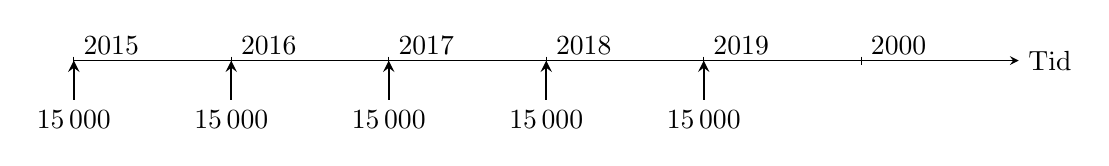
\begin{tikzpicture}[x=2cm,y=0.5cm,>=stealth]
  % Tidslinje
  \draw[->] (0,0) -- (6,0) node[right]{Tid};

  % Årstall
  \foreach \x \aar in {0/2015,1/2016,2/2017,3/2018,4/2019, 5/2000} {
    \draw (\x,0.1) -- (\x,-0.1) node[above right]{\aar};
  }
  % Innskudd
  \foreach \x in {0,1,2,3,4} {
    \draw[<-, thick] (\x,0) -- (\x,-1) node[below]{15\,000};
  }
\end{tikzpicture}
\end{center}

\end{frame}

\begin{frame}[t]{Eksempel: Hvor mye står på kontoen like etter siste innskudd}
\begin{center}
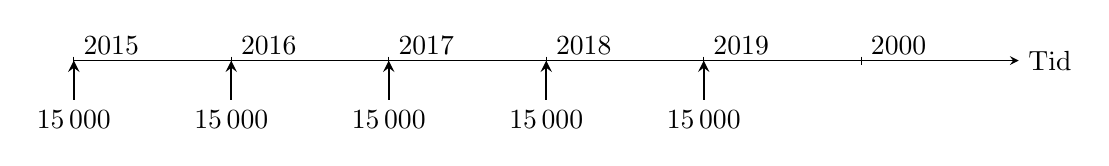
\begin{tikzpicture}[x=2cm,y=0.5cm,>=stealth]
  % Tidslinje
  \draw[->] (0,0) -- (6,0) node[right]{Tid};

  % Årstall
  \foreach \x \aar in {0/2015,1/2016,2/2017,3/2018,4/2019,5/2000} {
    \draw (\x,0.1) -- (\x,-0.1) node[above right]{\aar};
  }
  % Innskudd
  \foreach \x in {0,1,2,3,4} {
    \draw[<-, thick] (\x,0) -- (\x,-1) node[below]{15\,000};
  }
\end{tikzpicture}
\end{center}
\begin{columns}[T,onlytextwidth]
  \begin{column}{0.80\textwidth}
  \end{column}
   \begin{column}{0.20\textwidth}
    \begin{align*}
      &15\,000\cdot 1,034^0\\
      &15\,000\cdot 1,034^1\\
      &15\,000\cdot 1,034^2\\
      &15\,000\cdot 1,034^3\\
      &15\,000\cdot 1,034^4
    \end{align*}
\end{column}
\end{columns}
\end{frame}


\begin{frame}[t]{Eksempel: Hvor mye står på kontoen like etter siste innskudd}
\begin{center}
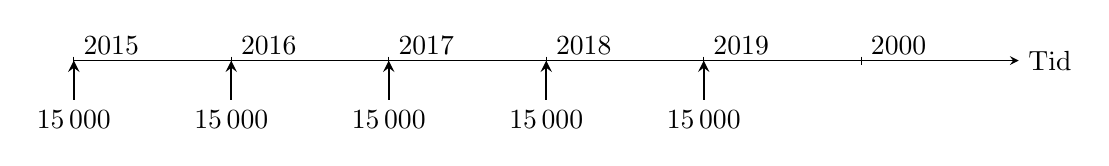
\begin{tikzpicture}[x=2cm,y=0.5cm,>=stealth]
  % Tidslinje
  \draw[->] (0,0) -- (6,0) node[right]{Tid};
  % Årstall
  \foreach \x \aar in {0/2015,1/2016,2/2017,3/2018,4/2019, 5/2000} {
    \draw (\x,0.1) -- (\x,-0.1) node[above right]{\aar};
  }
  % Innskudd
  \foreach \x in {0,1,2,3,4} {
    \draw[<-, thick] (\x,0) -- (\x,-1) node[below]{15\,000};
  }
\end{tikzpicture}
\end{center}
\begin{columns}[T,onlytextwidth]
  \begin{column}{0.80\textwidth}
  \begin{flalign*}
      &\\
      &\\
     s&=\sum_{n=1}^5 15\;000\cdot 1.034^{5-1}&\\
      &=15\;000\cdot \frac{1,034^5-1}{1,034-1}&\\
      &=80\;276,37
  \end{flalign*}
  \end{column}
   \begin{column}{0.20\textwidth}
    \begin{align*}
      &15\,000\cdot 1,034^0\\
      &15\,000\cdot 1,034^1\\
      &15\,000\cdot 1,034^2\\
      &15\,000\cdot 1,034^3\\
      &15\,000\cdot 1,034^4
    \end{align*}
\end{column}
\end{columns}
\end{frame}


\begin{comment}
\greenheader
\begin{frame}[fragile]{Eksempel: Hvor mye står på kontoen like etter siste innskudd?}

\begin{minted}[fontsize=\large]{python}
n = 5      # Antall inskudd
p = 1.034  # Rente per år
I = 15_000 # Årlig innskudd

# Første innskudd er 1. jauar 2015
# Siste innskudd er 1. januar 2019

# Bruker "list comprehension" for å lage talfølgen, minListe
minListe = [round(I*p**i) for i in range(n)]

print("Tallfølgen: ", minListe) 
# Output -> [15000, 15510, 16037, 16583, 17146]

print("Summen:", sum(minListe)) 
# Output -> Summen: 80276
\end{minted}
\end{frame}
\end{comment}

\begin{frame}[t]{Eksempel: Hvor mye står på kontoen 31. desember 2019?}
\begin{center}
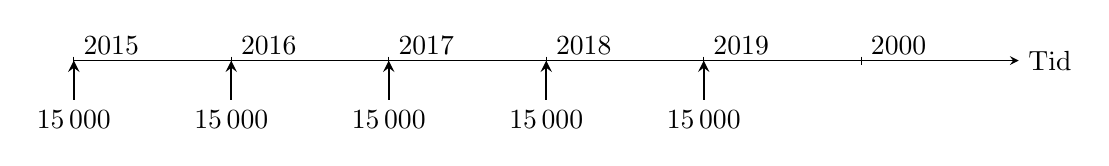
\begin{tikzpicture}[x=2cm,y=0.5cm,>=stealth]
  % Tidslinje
  \draw[->] (0,0) -- (6,0) node[right]{Tid};
  % Årstall
  \foreach \x \aar in {0/2015,1/2016,2/2017,3/2018,4/2019, 5/2000} {
    \draw (\x,0.1) -- (\x,-0.1) node[above right]{\aar};
  }
  % Innskudd
  \foreach \x in {0,1,2,3,4} {
    \draw[<-, thick] (\x,0) -- (\x,-1) node[below]{15\,000};
  }
\end{tikzpicture}
\end{center}
\begin{columns}[T,onlytextwidth]
  \begin{column}{0.80\textwidth}
  \begin{flalign*}
    &\\
    &\\
     s&=\sum_{n=1}^5 15\;000\cdot 1.034\cdot  1.034^{5-1}&\\
      &=15\;000\cdot1,034\cdot \frac{1,034^5-1}{1,034-1}&\\
      &=83\;005,76
  \end{flalign*}
  \end{column}
   \begin{column}{0.20\textwidth}
    \begin{align*}
      &15\,000\cdot 1,034^1\\
      &15\,000\cdot 1,034^2\\
      &15\,000\cdot 1,034^3\\
      &15\,000\cdot 1,034^4\\
      &15\,000\cdot 1,034^5
    \end{align*}
\end{column}
\end{columns}
\end{frame}


\begin{comment}
\greenheader
\begin{frame}[fragile]{Eksempel: Hvor mye står på kontoen 31. desember 2019?}
\begin{minted}[fontsize=\normalsize]{python}
n = 5      # Antall inskudd
p = 1.034  # Rente per år
I = 15_000 # Årlig innskudd

# Første inskudd er 1. jauar 2015
# Siste inskudd er 1. januar 2019

# Følge der første ledd er 15_000*1.034
minListe = [I*p*p**i for i in range(n)] 

print("Summen:", sum(minListe)) 
# Output -> Summen: 83005.76435177136

\end{minted}
\end{frame}
\end{comment}


\begin{frame}[t]{Eksempel: Hvor mye står på kontoen like etter siste innskudd?}
\begin{center}
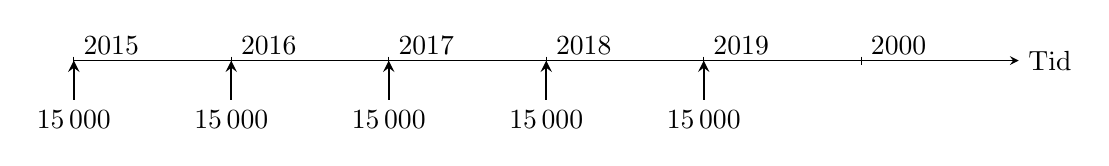
\begin{tikzpicture}[x=2cm,y=0.5cm,>=stealth]
  % Tidslinje
  \draw[->] (0,0) -- (6,0) node[right]{Tid};

  % Årstall
  \foreach \x \aar in {0/2015,1/2016,2/2017,3/2018,4/2019,5/2000} {
    \draw (\x,0.1) -- (\x,-0.1) node[above right]{\aar};
  }
  % Innskudd
  \foreach \x in {0,1,2,3,4} {
    \draw[<-, thick] (\x,0) -- (\x,-1) node[below]{15\,000};
  }
\end{tikzpicture}
\end{center}
\begin{columns}[T,onlytextwidth]
  \begin{column}{0.10\textwidth}
    \begin{align*}
      &\\
      &\\
      &15\,000 / 1,034^0\\
      &15\,000 / 1,034^1\\
      &15\,000 / 1,034^2\\
      &15\,000 / 1,034^3\\
      &15\,000 / 1,034^4
    \end{align*}
  \end{column}
   \begin{column}{0.90\textwidth}
\end{column}
\end{columns}
\end{frame}

\begin{frame}[t]{Eksempel: Hvor mye står på kontoen like etter siste innskudd?}
\begin{center}
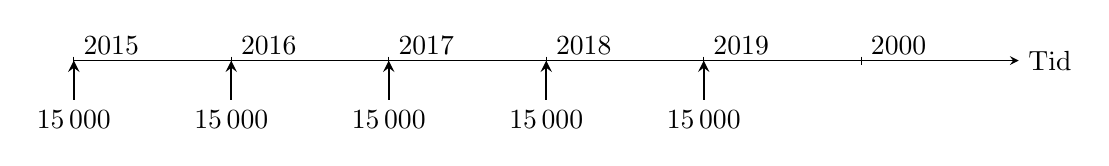
\begin{tikzpicture}[x=2cm,y=0.5cm,>=stealth]
  % Tidslinje
  \draw[->] (0,0) -- (6,0) node[right]{Tid};

  % Årstall
  \foreach \x \aar in {0/2015,1/2016,2/2017,3/2018,4/2019,5/2000} {
    \draw (\x,0.1) -- (\x,-0.1) node[above right]{\aar};
  }
  % Innskudd
  \foreach \x in {0,1,2,3,4} {
    \draw[<-, thick] (\x,0) -- (\x,-1) node[below]{15\,000};
  }
\end{tikzpicture}
\end{center}
\begin{columns}[T,onlytextwidth]
  \begin{column}{0.10\textwidth}
    \begin{align*}
      &\\
      &\\
      &15\,000 / 1,034^0\\
      &15\,000 / 1,034^1\\
      &15\,000 / 1,034^2\\
      &15\,000 / 1,034^3\\
      &15\,000 / 1,034^4
    \end{align*}
  \end{column}
  \begin{column}{0.30\textwidth}
  \end{column}
   \begin{column}{0.60\textwidth}
   \begin{align*}
     S_{2015}&=\sum_{n=1}^5 15\;000\cdot \left(\frac{1}{1.034}\right)^{5-1}\\
             &=15\;000\cdot \frac{\left(\frac{1}{1.034}\right)^5-1}{\frac{1}{1.034}-1}\\
             &=70\;227,23\\
     S_{2019}&=70\;227,23\cdot 1.034^4\\
             &=80\;276,37
   \end{align*}
\end{column}
\end{columns}
\end{frame}

\begin{frame}[t]{Eksempel: Hvor mye står på kontoen 31. desember 2019?}
\begin{center}
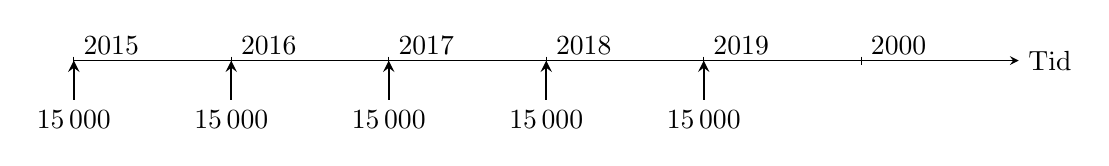
\begin{tikzpicture}[x=2cm,y=0.5cm,>=stealth]
  % Tidslinje
  \draw[->] (0,0) -- (6,0) node[right]{Tid};

  % Årstall
  \foreach \x \aar in {0/2015,1/2016,2/2017,3/2018,4/2019,5/2000} {
    \draw (\x,0.1) -- (\x,-0.1) node[above right]{\aar};
  }
  % Innskudd
  \foreach \x in {0,1,2,3,4} {
    \draw[<-, thick] (\x,0) -- (\x,-1) node[below]{15\,000};
  }
\end{tikzpicture}
\end{center}
\begin{columns}[T,onlytextwidth]
  \begin{column}{0.10\textwidth}
    \begin{align*}
      &\\
      &\\
      &15\,000 / 1,034^0\\
      &15\,000 / 1,034^1\\
      &15\,000 / 1,034^2\\
      &15\,000 / 1,034^3\\
      &15\,000 / 1,034^4
    \end{align*}
  \end{column}
  \begin{column}{0.30\textwidth}
  \end{column}
   \begin{column}{0.60\textwidth}
   \begin{align*}
     S_{2015}&=\sum_{n=1}^5 15\;000\cdot \left(\frac{1}{1.034}\right)^{5-1}\\
             &=15\;000\cdot \frac{\left(\frac{1}{1.034}\right)^5-1}{\frac{1}{1.034}-1}\\
             &=70\;227,23\\
     S_{2019}&=70\;227,23\cdot 1.034^5\\
             &=83\;005,76
   \end{align*}
\end{column}
\end{columns}
\end{frame}


\begin{comment}
\greenheader
\begin{frame}[fragile]{1E: Eksempel: Hvor mye står på kontoen 31. desember 2019?}
\begin{minted}[fontsize=\normalsize]{python}
n = 5      # Antall inskudd
p = 1.034  # Rente per år
I = 15_000 # Årlig innskudd

# Første inskudd er 1. jauar 2015
# Siste inskudd er 1. januar 2019

# Følge av nåverdier, første ledd er 15_000
nåverdierListe = [I/(p**i) for i in range(n)]

# Multipliserer summen med p**(n-1)
print("Summen:", sum(nåverdierListe)*p**(n-1))
# Output -> Summen: 80276.36784504
  
\end{minted}
\end{frame}
\end{comment}

\greenheader
\begin{frame}[t]{Eksempel: Annuitetslån}
\begin{center}
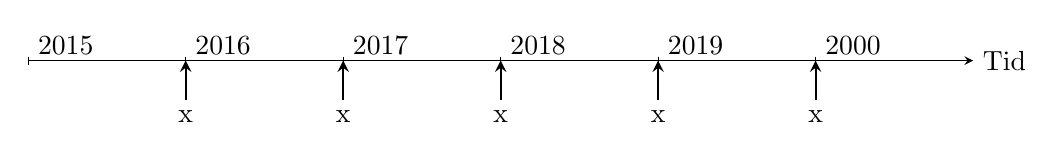
\begin{tikzpicture}[x=2cm,y=0.5cm,>=stealth]
  % Tidslinje
  \draw[->] (0,0) -- (6,0) node[right]{Tid};

  % Årstall
  \foreach \x \aar in {0/2015,1/2016,2/2017,3/2018,4/2019,5/2000} {
    \draw (\x,0.1) -- (\x,-0.1) node[above right]{\aar};
  }
  % Innskudd
  \foreach \x in {1,2,3,4,5} {
    \draw[<-, thick] (\x,0) -- (\x,-1) node[below]{x};
  }
\end{tikzpicture}
\end{center}
\medskip
\begin{itemize}
    \item Lånebeløp: $L=20\;000$ i januar 2015.\\
    \item Siste terminbeløp betales inn 31. desember 2019.
    \item Årlig rente: 7,4 \%. Vi setter $p=1,074$. 
    \item Årlig terminbeløp = $x$.
    \item Antall terminbeløp: 5.
\end{itemize}

\medskip
\textbf{Oppgave:} Finn størrelsen på det årlige terminbeløpet, $x$. 
\end{frame}

\greenheader
\begin{frame}[t]{Eksempel: Annuitetslån med sluttverdier}
\begin{center}
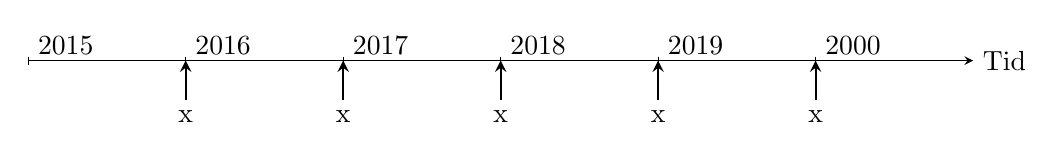
\begin{tikzpicture}[x=2cm,y=0.5cm,>=stealth]
  % Tidslinje
  \draw[->] (0,0) -- (6,0) node[right]{Tid};

  % Årstall
  \foreach \x \aar in {0/2015,1/2016,2/2017,3/2018,4/2019,5/2000} {
    \draw (\x,0.1) -- (\x,-0.1) node[above right]{\aar};
  }
  % Innskudd
  \foreach \x in {1,2,3,4,5} {
    \draw[<-, thick] (\x,0) -- (\x,-1) node[below]{x};
  }
\end{tikzpicture}
\end{center}
\begin{columns}[T,onlytextwidth]
  \begin{column}{0.50\textwidth}
  \begin{flalign*}
  &\\
  &\\
  &\\
      \sum_{n=1}^5 x\cdot 1,074^{n-1}&=20\;000\cdot 1.074^5\\
      x\cdot \frac{1,074^5-1}{1,074-1}&=20\;000\cdot 1.074^5\\
  \end{flalign*}
  \end{column}
  \begin{column}{0.20\textwidth}
  \end{column}
   \begin{column}{0.30\textwidth}
    \begin{align*}
      &\\
      &\\
      &x\cdot 1,074^0\\
      +\;&x\cdot 1,074^1\\
      +\;&x\cdot 1,074^2\\
      +\;&x\cdot 1,074^3\\
     +\;&x\cdot 1,074^4\\
      =\;&20\;000\cdot 1.074^5
    \end{align*}
\end{column}
\end{columns}
\end{frame}

\greenheader
\begin{frame}[t]{Eksempel: Annuitetslån med sluttverdier}
\begin{center}
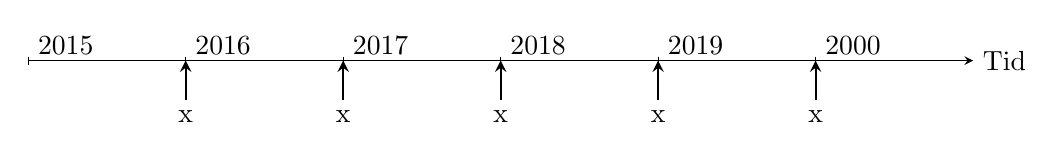
\begin{tikzpicture}[x=2cm,y=0.5cm,>=stealth]
  % Tidslinje
  \draw[->] (0,0) -- (6,0) node[right]{Tid};

  % Årstall
  \foreach \x \aar in {0/2015,1/2016,2/2017,3/2018,4/2019,5/2000} {
    \draw (\x,0.1) -- (\x,-0.1) node[above right]{\aar};
  }
  % Innskudd
  \foreach \x in {1,2,3,4,5} {
    \draw[<-, thick] (\x,0) -- (\x,-1) node[below]{x};
  }
\end{tikzpicture}
\end{center}
\begin{columns}[T,onlytextwidth]
  \begin{column}{0.70\textwidth}
 \begin{figure}
      \centering
      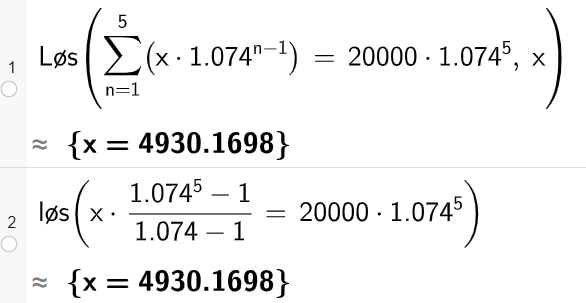
\includegraphics[width=0.8\linewidth]{R2K1E-1.png}
  \end{figure}
  \end{column}
   \begin{column}{0.30\textwidth}
    \begin{align*}
      &\\
      &\\
      &x\cdot 1,074^0\\
      +\;&x\cdot 1,074^1\\
      +\;&x\cdot 1,074^2\\
      +\;&x\cdot 1,074^3\\
     +\;&x\cdot 1,074^4\\
      =\;&20\;000\cdot 1.074^5
    \end{align*}
\end{column}
\end{columns}
\end{frame}

\greenheader
\begin{frame}[t]{Eksempel: Annuitetslån med nåverdier}
\begin{center}
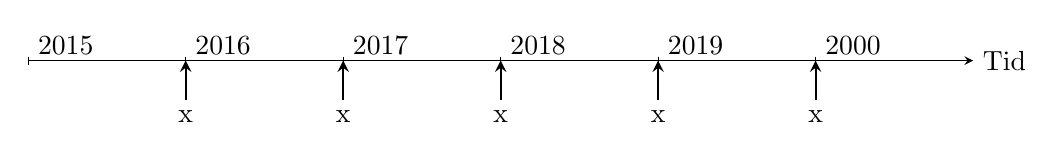
\begin{tikzpicture}[x=2cm,y=0.5cm,>=stealth]
  % Tidslinje
  \draw[->] (0,0) -- (6,0) node[right]{Tid};

  % Årstall
  \foreach \x \aar in {0/2015,1/2016,2/2017,3/2018,4/2019,5/2000} {
    \draw (\x,0.1) -- (\x,-0.1) node[above right]{\aar};
  }
  % Innskudd
  \foreach \x in {1,2,3,4,5} {
    \draw[<-, thick] (\x,0) -- (\x,-1) node[below]{x};
  }
\end{tikzpicture}
\end{center}
\begin{columns}[T,onlytextwidth]
\begin{column}{0.20\textwidth}
 \begin{align*}
      &x/ 1,074^1\\
      +\;&x/1,074^2\\
      +\;&x/ 1,074^3\\
      +\;&x/ 1,074^4\\
     +\;&x/ 1,074^5\\
      =\;&20\;000
    \end{align*}
  \end{column}
  \begin{column}{0.30\textwidth}
\end{column}
\begin{column}{0.50\textwidth}
\begin{flalign*}
  &\\
  &\\
      \sum_{n=1}^5 \frac{x}{1,074}\cdot \left(\frac{1}{1,074}\right)^{n-1}&=20\;000\\
      \frac{x}{1,074} \cdot \frac{\left(\frac{1}{1,074}\right)^5-1}{\frac{1}{1,074}-1}&=20\;000\\
  \end{flalign*}
\end{column}
\end{columns}
\end{frame}

\greenheader
\begin{frame}[t]{Eksempel: Annuitetslån med nåverdier}
\begin{center}
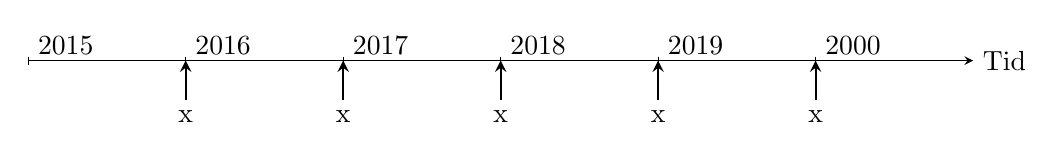
\begin{tikzpicture}[x=2cm,y=0.5cm,>=stealth]
  % Tidslinje
  \draw[->] (0,0) -- (6,0) node[right]{Tid};

  % Årstall
  \foreach \x \aar in {0/2015,1/2016,2/2017,3/2018,4/2019,5/2000} {
    \draw (\x,0.1) -- (\x,-0.1) node[above right]{\aar};
  }
  % Innskudd
  \foreach \x in {1,2,3,4,5} {
    \draw[<-, thick] (\x,0) -- (\x,-1) node[below]{x};
  }
\end{tikzpicture}
\end{center}
\begin{columns}[T,onlytextwidth]
\begin{column}{0.20\textwidth}
 \begin{align*}
      &x/ 1,074^1\\
      +\;&x/1,074^2\\
      +\;&x/ 1,074^3\\
      +\;&x/ 1,074^4\\
     +\;&x/ 1,074^5\\
      =\;&20\;000
    \end{align*}
  \end{column}
\begin{column}{0.80\textwidth}
\begin{figure}
    \centering
    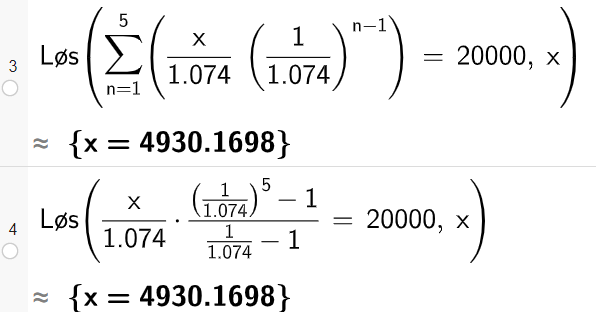
\includegraphics[width=0.7\linewidth]{R2K1E-2.png}
\end{figure}
\end{column}
\end{columns}
\end{frame}


